\ylDisplay{Elektron} % Ülesande nimi
{Mihkel Kree} % Autor
{lahtine} % Voor
{2017} % Aasta
{G 3} % Ülesande nr.
{4} % Raskustase
{
% Teema: Elektrostaatika
\ifStatement
\begin{wrapfigure}[7]{r}{0.5\linewidth}
	\vspace{-10pt}
	\hspace{-10pt}
	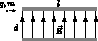
\includegraphics[width=\linewidth]{2017-lahg-03-elJoonisMK.pdf}
\end{wrapfigure}

Elektron liigub vaakumis ning siseneb paralleelsete plaatide vahel paiknevasse ruumipiirkonda selle ülemisest servast nii, et elektroni kiirusvektor on paralleelne plaatidega (vt joonist). Kui suur on elektroni minimaalne võimalik kiirus $v_\mathrm{min}$ plaatide vahelisest ruumipiirkonnast väljumisel? Plaatide pikkus on $l$ ja nende vahekaugus $d$. Plaatide vahel on ühtlane elektriväli $\vec{E}$ ning ääreefektidega pole vaja arvestada. Elektroni laeng on $q$ ning mass $m$. Gravitatsioonijõuga pole vaja arvestada.
\fi


\ifHint
Plaatide vahel mõjub elektronile elektrivälja poolt allapoole suunatud kiirendus. Seega on elektroni kiirus plaatide vahelisest ruumist väljumisel minimaalne siis, kui elektroni trajektoor möödub alumise plaadi parema otsa lähedalt.
\fi


\ifSolution
Elektriväljas liikuvale elektronile mõjub allapoole suunatud vertikaalne jõud $qE$, millele vastab elektroni kiirendus $a=qE/m$. Seega võime elektroni liikumist analüüsida analoogiliselt õhku visatud kivi liikumisega: a) elektron liigub mööda paraboolselt trajektoori; b) elektroni kiiruse horisontaalkomponent $v_0$ ei muutu; c) elektroni kiiruse vertikaalkomponent kasvab ajas kujul $v_y=at$; d) elektroni horisontaalne nihe kasvab ajas kujul $x=v_0t$; e) elektroni vertikaalne nihe kasvab ajas kujul $y=at^2/2$.

Elektroni kiirus plaatide vahelisest ruumist väljumisel on minimaalne siis, kui elektroni trajektoor möödub alumise plaadi parema otsa lähedalt. Sellest väiksema kiiruse korral lendaks elektron vastu alumist plaati ning ei pääseks seetõttu plaatide vahelisest ruumist välja.

Olgu elektroni algkiirus $v_0$. Elektronil kulub plaatide vahelise ruumi läbimiseks aeg $t=l/v_0$, mille jooksul peab vertikaalne nihe olema võrdne plaatide vahelise kaugusega $d=at^2/2$. Siit saame avaldada elektroni plaatide vahel liikumise aja $t=\sqrt{2d/a}$, elektroni vertikaalse kiiruse plaatide vahelisest ruumist väljumisel $v_y=at=\sqrt{2ad}$ ning elektroni minimaalse vajaliku algkiiruse $v_0=l/t=\sqrt{al^2/2d}$. Nüüd saame avaldada otsitava minimaalse lõppkiiruse mooduli:
\[
v_\mathrm{min}=\sqrt{v_y^2+v_0^2}=\sqrt{2ad+\frac{al^2}{2d}}=\sqrt{\frac{qE\left(4d^2+l^2\right)}{2md}}.
\]
\fi


\ifEngStatement
% Problem name: Electron
\begin{wrapfigure}[7]{r}{0.5\linewidth}
	\vspace{-10pt}
	\hspace{-10pt}
	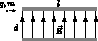
\includegraphics[width=\linewidth]{2017-lahg-03-elJoonisMK}
\end{wrapfigure}
An electron is moving in vacuum and enters a region of space between parallel plates from the area’s upper edge so that the electron’s velocity is parallel to the plates (see figure). How big is the electron’s minimal possible speed $v_\mathrm{min}$ when exiting the area of space between the plates? The length of the plates is $l$ and the distance between them is $d$. Between the plates there is a homogeneous electric field $\vec{E}$, neglect edge effects. The electron’s charge is $q$ and its mass is $m$. Neglect the gravitational force.
\fi


\ifEngHint
Between the plates a downwards directed acceleration is applied to the electron by the electric field. Thus the speed of the electron when exiting the room area between the plates is minimal in the case where the electron's trajectory passes close to the bottom plate's right tip.
\fi


\ifEngSolution
The electron moving in the electric field is affected by a vertical force $qE$ directed downwards and has the respective acceleration $a=qE/m$. Therefore we can analyze the electron’s movement the same way as the movement of a stone that is thrown into air: a) the electron is moving along a parabolic trajectory; b) the horizontal component $v_0$ of the electron’s velocity does not change; c) the vertical component of the electron’s velocity increases in time as $v_y=at$; d) the horizontal displacement of the electron increases in time as $x=v_0t$; e) the vertical displacement of the electron increases in time as $y=at^2/2$.\\
The electron’s velocity when exiting the space between the plates is minimal when the electron’s trajectory passes close to the right corner of the bottom plate. Below this velocity the electron would fly against the bottom plate and would not therefore manage to get out of the space between the plates.\\
Let the initial velocity of the electron be $v_0$. The time it takes the electron to go through the space between the plates is $t=l/v_0$ during which the vertical displacement has to be equal to the distance $d=at^2/2$ between the plates. From this we can express the time the electron moves between the plates $t=\sqrt{2d/a}$, the vertical velocity of the electron when exiting the space between the plates $v_y=at=\sqrt{2ad}$ and the minimal initial velocity of the electron $v_0=l/t=\sqrt{al^2/2d}$. Now we can express the module of the desired minimal final velocity:
\[
v_\mathrm{min}=\sqrt{v_y^2+v_0^2}=\sqrt{2ad+\frac{al^2}{2d}}=\sqrt{\frac{qE\left(4d^2+l^2\right)}{2md}}.
\]
\fi
}